\chapter{Methodology and System Design}

\section{Introduction}
The methods and procedures used to design the ShopSense platform, as well as the system architecture and key components, are described in this chapter. The software process model used for the project is first described, followed by the functional and non-functional requirements, the overall system architecture, and the detailed design of the backend, frontend, AI components, and payment subsystems.Lastly, it discusses the important performance and security factors that influenced the design choices.

\section{Software Process Model and Methodology}

We build Shopsense using an iterative similar methodthe  like agile method instead of the waterfall method.The work was divided into phases in accordance with the Gantt chart in Chapter 1 (Figure~\ref{fig:gantt-chart}), with each phase providing an incremental set of features:


\begin{itemize}
  \item \textbf{Phase 1: Planning and Requirements-} Analysis of current e-commerce sites, literature review, and definition of functional and non-functional requirements.
  \item \textbf{Phase 2: Core Platform Development-} Implementation of core Django Database classes, REST APIs Endpoints, and basic static pages for products, cart, and orders.
  \item \textbf{Phase 3: Payments and Advanced Features-} Integration coupon system, different payment methods like MFS and Card payment and fine tuning of checkout flows.
  \item \textbf{Phase 4: AI/ML Components} Development of semantic search, recommendation engine, and chat-bot using Lang-Chain and ChromaDB.
  \item \textbf{Phase 5: Testing and Deployment-} Functional testing, performance checks on key workflows, and deployment configuration on a cloud platform.
\end{itemize}

The team evaluated progress at the conclusion of each phase, noted problems, and modified the backlog of work for following iterations.This methodical approach approach allowed for early validation of key functionality (such as basic cart and checkout) prior to investing in more sophisticated AI features, and also enabled design modifications depending on implementation and testing outcomes.

\section{System Requirements}
The functional and non-functional needs of the \textit{ShopSense: Intelligent E-Commerce Platform} are described in this section. The issue statement, literature analysis, and observation of standard procedures in already-existing online stores were used to determine the needs.


\subsection{Functional Requirements}
Functional requirements outline what the system must accomplish from the viewpoints of administrators, clients, and AI services.

\subsubsection*{Customer-related Requirements}
\begin{itemize}
  \item \textbf{User registration and login:} The system must enable users to register, log in, and keep a personal profile with basic data and stored addresses.
  \item \textbf{Product browsing:} The system will provide products arranged by categories and sub-categories, supporting sorting (e.g., most-viewed, price, popularity) and filtering (e.g., category).
  \item \textbf{Product details:} The system must offer a comprehensive product view that includes stock information, available variations (such as size and color), price, description, and photos.
  \item \textbf{Shopping cart management:} Customers should be able to add products to their cart, change quantities, delete things, and display a summary of their cart that includes discounts and subtotals.
  \item \textbf{Checkout process:} Customers can enter or choose shipping addresses, select a payment option, and examine the order before confirmation using the system's multi-step checkout flow.
  \item \textbf{Order placement and tracking:} Following a successful checkout, the system will establish orders and enable consumers to monitor order history and current order status.
  \item \textbf{Coupon usage:} Customers will be able to apply valid coupon codes to qualifying orders and see the resultant discounts.
  \item \textbf{Payment options:} The system must accept a variety of payment methods, such as card payments via Stripe, mobile payments via bKash, and cash on delivery (COD), with clear indications of fees or restrictions where relevant.
  \item \textbf{AI chat-bot assistance:} After the user has been authorized, the system will offer an AI-powered chat-bot that can respond to inquiries about the product, help with navigation (such as locating goods by criteria), and provide basic order details.
  \item \textbf{Semantic search:} Customers can use natural language queries to search for products, and even if the query does not precisely match product titles, the system returns results that are semantically relevant.
  \item \textbf{Recommendations:} On pertinent sites, the system will provide tailored or context-aware product recommendations, such as "related products" and "customers also viewed."
\end{itemize}

\subsubsection*{Administrator and Staff Requirements}
\begin{itemize}
  \item \textbf{Product management:} Using a backend interface, administrators add, modify, and remove products, categories, and subcategories.
  \item \textbf{Inventory management:} Administrators manage stock levels and indicate whether a product is active or inactive.
  \item \textbf{Order management:} Administrators examine payment details, inspect orders, and adjust order status (such as pending, paid, shipped, delivered, or canceled).
  \item \textbf{Coupon management:} Administrators generate and oversee coupon codes, including their discount type, value, expiration date, and usage restrictions.
  \item \textbf{User management:} Administrators examine registered users, change roles as needed, and deal with account-related problems.
  \item \textbf{Analytics and reports (basic):} To aid in decision-making, the system offers fundamental indicators including the quantity of orders, total revenue, popular products, and coupon utilization.
\end{itemize}

\subsubsection*{AI and Integration Requirements}
\begin{itemize}
  \item \textbf{Product data ingestion:} Product information will be ingested into the AI as resources (vector database, recommendation engine) to get updated data from searches and recommendations.
  \item \textbf{Chat-bot backend selection:} Customizable chatbot backends, including local LLM (via Ollama) and a mock or external provider, will be supported and can be changed by environmental variables.
  \item \textbf{Payment gateway integration:} The system shall integrate with Stripe and
bKash APIs for payment initialization, status verification, and web-hook handling.
  \item \textbf{API access:} The platform shall expose REST APIs for cart operations, product
retrieval, recommendations, coupon validation, and chat-bot communication
to support the Vue.js front-end and possible future clients.
\end{itemize}

\subsection{Non-Functional Requirements (Performance, Security, Usability)}
Non-functional requirements describe constraints and quality attributes that the system should satisfy.

\subsubsection*{Performance Requirements}
\begin{itemize}
  \item The system shall respond to typical page requests (home page, catalog, product detail) within an acceptable time under normal load (e.g., target $< 1.5$ seconds server response time on a mid-range hosting environment).
  \item Semantic search and recommendation queries shall be optimized to return results within a practical latency budget (e.g., target $< 1$ second additional delay for search results).
  \item The platform shall efficiently handle concurrent users typical of a small to medium-sized store; heavy load or large-scale optimization is considered future work.
\end{itemize}

\subsubsection*{Security Requirements}
\begin{itemize}
  \item All authenticated pages and APIs shall enforce secure session management and authorization checks to prevent unauthorized access to user or administrative data.
  \item The system shall protect against common web vulnerabilities such as SQL injection, cross-site scripting (XSS), and cross-site request forgery (CSRF) using Django’s built-in security mechanisms and secure coding practices.
  \item Sensitive configuration values, such as secret keys and API credentials for Stripe and bKash, shall be stored in environment variables and not hardcoded in the source code.
  \item Payment card data shall never be stored on the application server; Stripe’s client-side or hosted checkout solutions shall be used so that payment data is processed directly by the gateway.
\end{itemize}

\subsubsection*{Usability and Reliability Requirements}
\begin{itemize}
  \item A good website is one that has seamless optimization for all devices, device dependency should not be a barrier to user experience, and design consistency is a must for user comfort.
  \item Proper error description and details make users more comfortable while facing any error in the web app. Proper guidance or hints can be useful to make users navigate more willingly.
  \item The system should log important events (e.g., payment callbacks, failed payments, order status changes) to support debugging and operational monitoring.
  \item The platform should provide proper error message when AI-features are unavailable (e.g., fallback to keyword search or mock chat-bot responses).
\end{itemize}

\section{System Design and Architecture}
This chapter described the methodology and system design of the ShopSense platform. An iterative, Agile-inspired process was adopted to develop the system in phases, guided by clearly defined functional and non-functional requirements.

\subsection{High-Level Architecture Diagram (Django + Vue + APIs + DB)}
A modular, service-oriented design is followed by the ShopSense architecture (Figure~\ref{fig:high-level-architecture}). The Django backend is communicated with by the Vue.js frontend through RESTful APIs. The relational database is interacted with by the backend for transactional data, and AI components are utilized for search, recommendations, and chatbot responses. Secure HTTP APIs and webhooks integrate payment gateways (Stripe and bKash).

\begin{figure}[H]
  \centering
  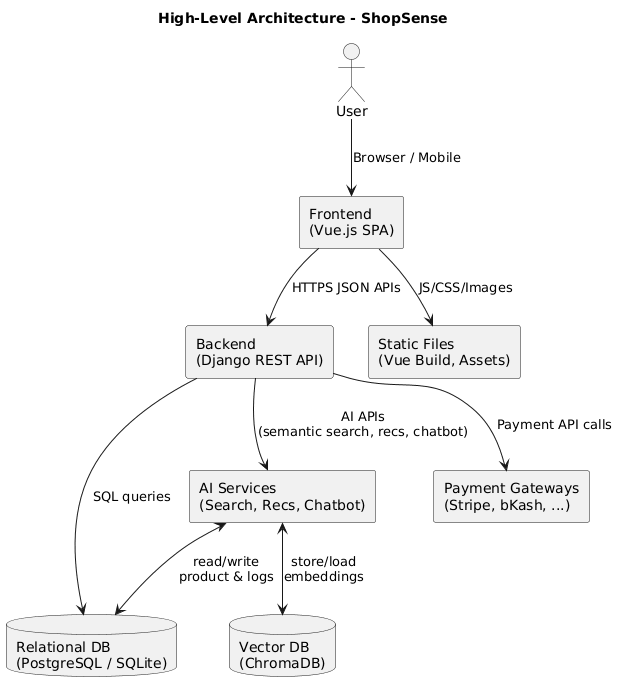
\includegraphics[width=0.9\textwidth]{Images/MyFigs/High-level architecture of the ShopSense.png}
  \caption{High-level architecture of the ShopSense platform, in which interactions among the Vue.js front end, Django backend, relational database, AI services, and payment gateways are visualized.}
  \label{fig:high-level-architecture}
\end{figure}

\subsection{Data Flow Between Front-end, Backend, and AI Services}
The primary data flows in the system are illustrated in Figure~\ref{fig:data-flow-frontend-backend-ai}. HTTP requests from the Vue.js front-end to the Django REST API are initiated by typical user actions—such as searching for products, viewing recommendations, or interacting with the chat-bot. Coordination with the relational database and AI services is then handled by the backend as needed.


\begin{itemize}
  \item \textbf{Product browsing and search:} The frontend sends search queries and filter parameters to the backend. For semantic search, the backend encodes the query into an embedding, queries the vector database, and returns ranked products to the frontend.
  \item \textbf{Chatbot interaction:} The frontend sends user messages to a chatbot API endpoint. The backend constructs a context, retrieves relevant product or documentation snippets via ChromaDB, forwards the prompt to the configured LLM backend (Ollama or external), and returns a generated response.
  \item \textbf{Recommendations:} When a user opens a product page or the cart, the frontend requests recommendations. The backend computes or retrieves recommended products using a hybrid strategy and returns them to be displayed alongside the primary content.
\end{itemize}

\begin{figure}[H]
  \centering
  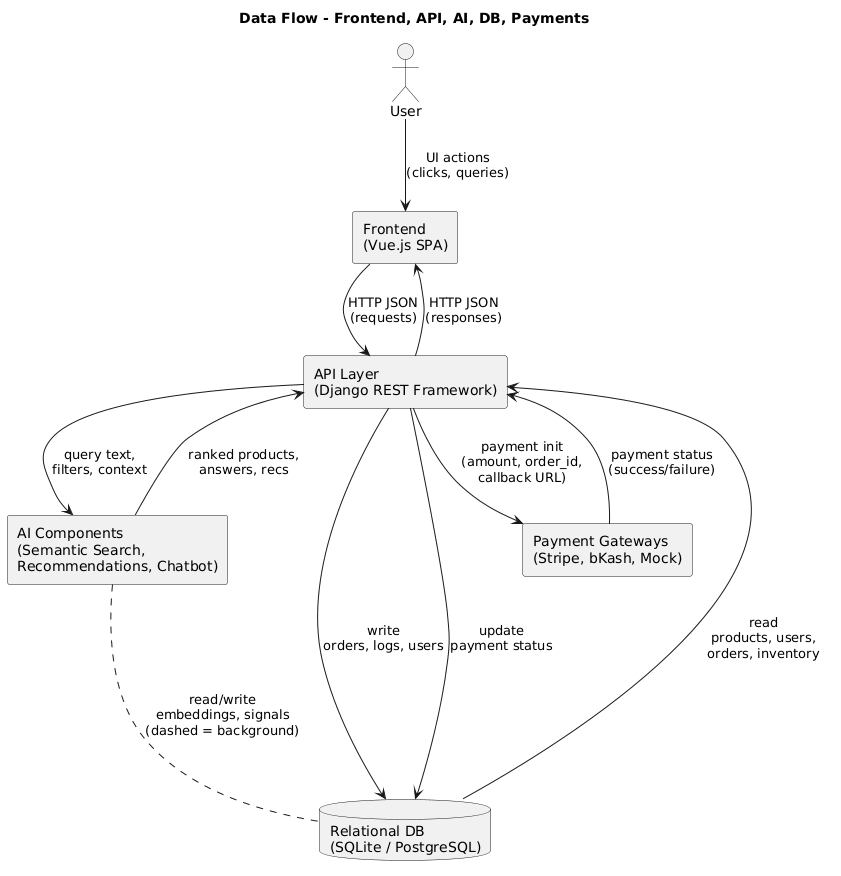
\includegraphics[width=0.9\textwidth]{Images/MyFigs/DataFlow-Frontend-API-AI-DB.png}
  \caption{Data flow between the Vue.js frontend, Django REST API, AI components (semantic search, recommendations, chatbot), and the relational database.}
  \label{fig:data-flow-frontend-backend-ai}
\end{figure}

\section{Backend Design (Django)}
The backend is implemented using Django and Django REST Framework. It is organized into multiple Django apps corresponding to core business domains, such as products, orders, cart, coupons, search, recommendations, and chatbot.

\subsection{Database Schema and Models (Products, Users, Orders, Cart, Coupons)}
The database schema follows a relational model using Django’s ORM. The key entities are illustrated in Figure~\ref{fig:erd-shopsense}.

\begin{figure}[H]
  \centering
  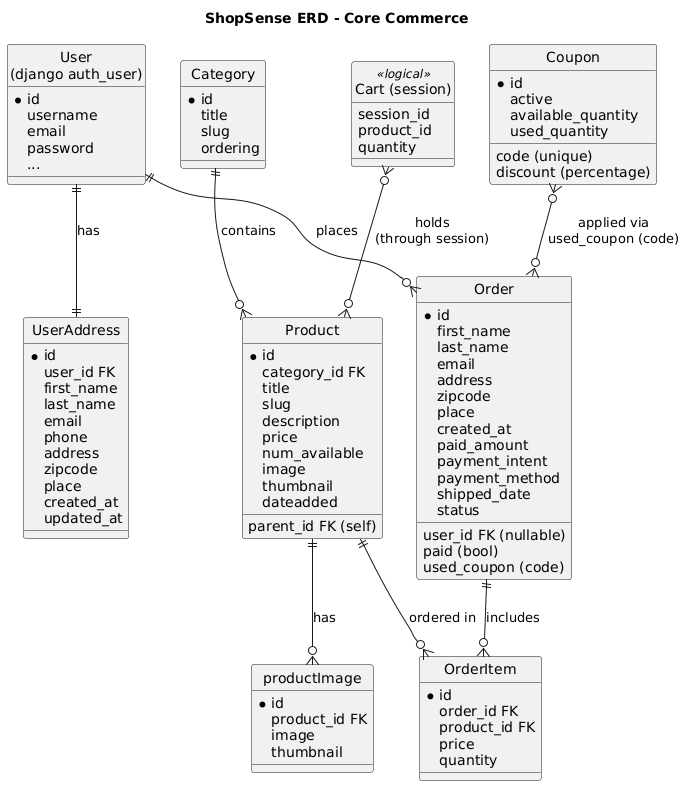
\includegraphics[width=0.9\textwidth]{Images/MyFigs/ShopSense ERD - Core Commerce.png}
  \caption{Entity--relationship diagram of the ShopSense database schema, including users, products, categories, carts, orders, order items, and coupons.}
  \label{fig:erd-shopsense}
\end{figure}

\subsubsection*{Core Entities}
\begin{itemize}
  \item \textbf{User:} Extends Django’s built-in user model (or uses a custom user model) to store customer information such as name, email, and addresses.
  \item \textbf{Category:} Represents high-level product categories and optional subcategories for organizing the catalog.
  \item \textbf{Product:} Stores product attributes including title, description, price, stock quantity, category, image paths, and optional variant information.
  \item \textbf{Cart and CartItem:} Represent a user’s active shopping cart and its items, with references to products and quantities. Sessions are used for anonymous carts when users are not logged in.
  \item \textbf{Order and OrderItem:} Capture confirmed purchases, linking users, products, quantities, applied discounts, payment status, and shipping information.
  \item \textbf{Coupon:} Represents discount codes with fields such as code, discount type (percentage or fixed amount), value, expiration date, minimum order amount, and usage limits.
  \item \textbf{Payment:} Stores payment-related metadata (transaction IDs, gateway type, status) received from Stripe, bKash, or the mock gateway.
\end{itemize}

\subsection{REST API Endpoints (Cart API, Product API, Recommendations API, Coupon API)}
The Django REST Framework is used to implement a set of JSON APIs consumed by the Vue.js frontend. Table~\ref{tab:api-overview} summarizes the main endpoints.

\begin{table}[H]
  \centering
  \caption{Overview of key REST API endpoints in the ShopSense backend.}
  \label{tab:api-overview}
  \begin{tabular}{p{4.5cm}p{2cm}p{6.5cm}}
    \toprule
    \textbf{Endpoint} & \textbf{Method(s)} & \textbf{Description} \\
    \midrule
    \texttt{/api/products/} & GET & List products with pagination, filters, and sorting. \\
    \midrule
    \texttt{/api/products/\{id\}/} & GET & Retrieve details of a single product. \\
    \midrule
    \texttt{/api/search/semantic/} & POST & Perform semantic search over the product catalog. \\
    \midrule
    \texttt{/api/cart/} & GET, POST & Retrieve current cart; add items to cart. \\
    \midrule
    \texttt{/api/cart/update/} & POST & Update quantities of items in the cart. \\
    \midrule
    \texttt{/api/cart/remove/} & POST & Remove items from the cart. \\
    \midrule
    \texttt{/api/cart\_count/} & GET & Return the number of items in the cart. \\
    \midrule
    \texttt{/api/recommendations/\newline\{product\_id\}/} & GET & Retrieve recommended products related to a given product. \\
    \midrule
    \texttt{/api/coupons/validate/} & POST & Validate coupon code and return discount information. \\
    \midrule
    \texttt{/api/checkout/initiate/} & POST & Initiate checkout and start payment flow. \\
    \midrule
    \texttt{/api/chatbot/message/} & POST & Send user message to chatbot and receive response. \\
    \bottomrule
  \end{tabular}
\end{table}

% \begin{table}[H]
%   \centering
%   \caption{Overview of key REST API endpoints in the ShopSense backend.}
%   \label{tab:api-overview}
%   \begin{tabular}{p{3cm}p{3cm}p{7cm}}
%     \toprule
%     \textbf{Endpoint} & \textbf{Method(s)} & \textbf{Description} \\
%     \midrule
%     \texttt{/api/products/} & GET & List products with pagination, filters, and sorting. \\
%     \texttt{/api/products/\{id\}/} & GET & Retrieve details of a single product. \\
%     \texttt{/api/search/semantic/} & POST & Perform semantic search over the product catalog. \\
%     \texttt{/api/cart/} & GET, POST & Retrieve current cart; add items to cart. \\
%     \texttt{/api/cart/update/} & POST & Update quantities of items in the cart. \\
%     \texttt{/api/cart/remove/} & POST & Remove items from the cart. \\
%     \texttt{/api/cart\_count/} & GET & Return the number of items in the cart. \\
%     \texttt{/api/recommendations/\{product\_id\}/} & GET & Retrieve recommended products related to a given product. \\
%     \texttt{/api/coupons/validate/} & POST & Validate coupon code and return discount information. \\
%     \texttt{/api/checkout/initiate/} & POST & Initiate checkout and start payment flow. \\
%     \texttt{/api/chatbot/message/} & POST & Send user message to chatbot and receive response. \\
%     \bottomrule
%   \end{tabular}
% \end{table}

Additional endpoints are provided for user registration, authentication, order retrieval, and administrative operations as required.

\section{Frontend Design (Vue.js)}
The frontend is implemented as a single-page application using Vue.js. It consumes the Django REST API and provides a responsive, interactive user interface.

\subsection{Component Structure (Home, Catalog, Product Detail, Cart, Checkout, Profile)}
The main view components are organized according to major user tasks, as depicted in Figure~\ref{fig:frontend-component-structure}:

\begin{itemize}
  \item \textbf{HomeView:} Landing page showcasing featured products, categories, promotional banners, and entry points to search and recommendations.
  \item \textbf{CatalogView:} Displays products by category with filtering, sorting, and pagination controls.
  \item \textbf{ProductDetailView:} Shows detailed information for a single product, including gallery, variants, reviews (if implemented), and a section for related products.
  \item \textbf{CartView:} Displays current cart items, quantities, subtotal, applied coupons, and options to update or remove items.
  \item \textbf{CheckoutView:} Implements the stepwise checkout process (address, payment method selection, order review).
  \item \textbf{ProfileView:} Allows users to view and update profile information, manage saved addresses, and see order history.
  \item \textbf{ChatbotWidget:} Provides a floating chat interface that can be opened from any page to interact with the AI assistant.
\end{itemize}

\begin{figure}[H]
  \centering
  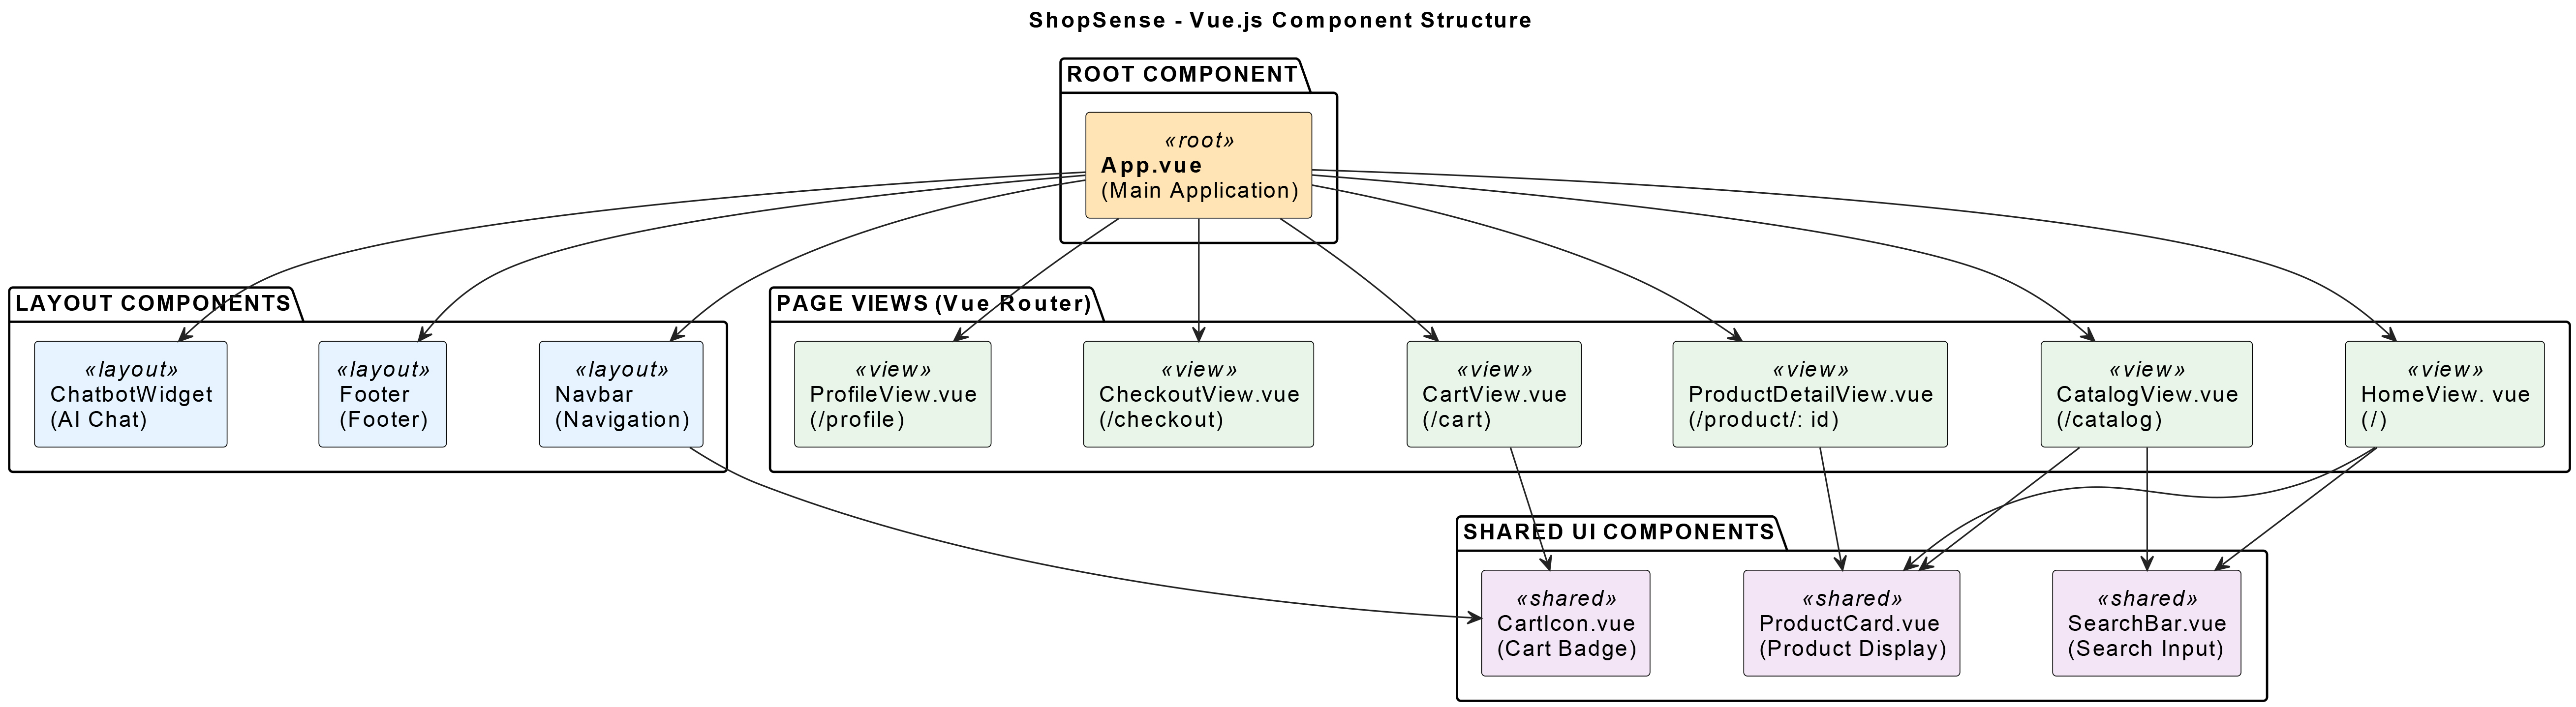
\includegraphics[width=0.9\textwidth]{Images/MyFigs/Simplified Vue.js Component Structure - ShopSense.jpg}
  \caption{Simplified Vue.js component structure for the ShopSense frontend.}
  \label{fig:frontend-component-structure}
\end{figure}

\subsection{State Management (Vuex) and Routing}
Application-level state such as the shopping cart, authenticated user information, and some UI preferences is managed using Vuex (or the equivalent state management library used in the implementation). Separate Vuex modules are used for:
\begin{itemize}
  \item \textbf{auth:} Handles authentication tokens, login/logout actions, and user profile data.
  \item \textbf{cart:} Stores cart items, counts, and computed totals; synchronizes with backend cart APIs.
  \item \textbf{products:} Caches product lists and product details to reduce redundant API calls.
  \item \textbf{chatbot:} Maintains current conversation state and last responses from the chatbot API.
\end{itemize}

Routing is managed using the Vue router, mapping URL paths to view components (e.g., \texttt{/}, \texttt{/catalog}, \texttt{/product/:id}, \texttt{/cart}, \texttt{/checkout}, \texttt{/profile}). Navigation guards are used to ensure that only authenticated users can access protected routes such as the profile and order history pages.

\section{AI Components}
The AI layer of ShopSense consists of three main components: the chatbot, the semantic search system, and the recommendation engine. These components share some underlying infrastructure, such as embedding models and the vector database.

\subsection{Chatbot Architecture (LangChain + Ollama/OpenAI + ChromaDB)}
The chatbot is implemented as a retrieval-augmented generation system (Figure~\ref{fig:chatbot-architecture}). Key elements include:
\begin{itemize}
  \item \textbf{Frontend chat widget:} Captures user messages and displays responses.
  \item \textbf{Chatbot API endpoint:} Receives messages from the frontend, attaches user/session metadata, and orchestrates the conversation logic.
  \item \textbf{Retrieval layer:} Uses ChromaDB to retrieve relevant product descriptions, FAQs, and documentation sections based on an embedding of the user query.
  \item \textbf{LLM backend:} Uses either a local LLM via Ollama or a remote LLM provider (e.g., OpenAI), selected through configuration.
  \item \textbf{Response generation:} Combines retrieved context documents with the user query in a prompt template and generates a response, which is then returned to the frontend.
\end{itemize}

\begin{figure}[H]
  \centering
  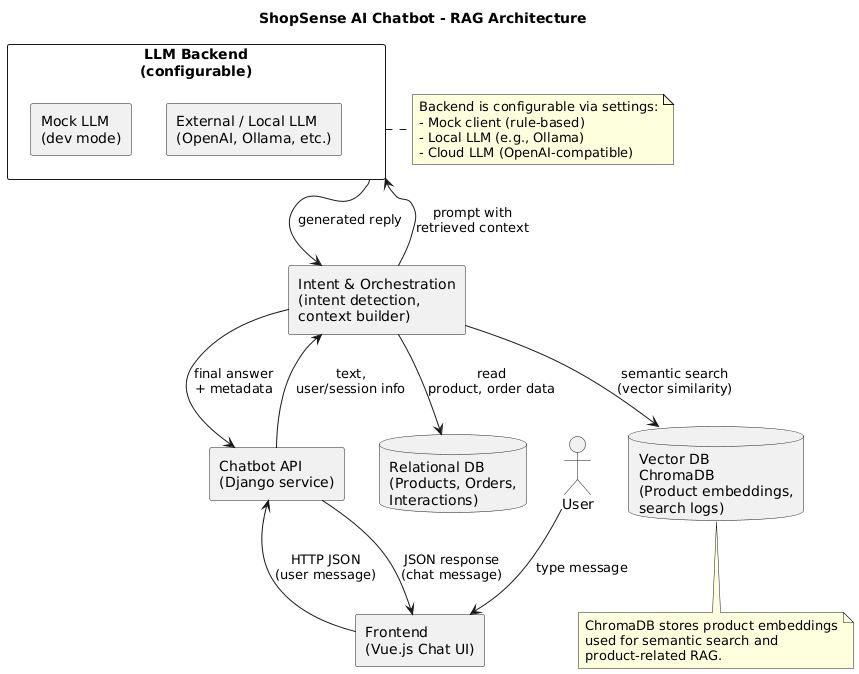
\includegraphics[width=0.9\textwidth]{Images/MyFigs/ShopSense AI Chatbot - RAG Architecture.png}
  \caption{Architecture of the ShopSense AI chatbot using retrieval-augmented generation with ChromaDB and configurable LLM backends.}
  \label{fig:chatbot-architecture}
\end{figure}

\subsection{Semantic Search System (Sentence Transformers, Vector Index)}
The semantic search system encodes product text (titles, descriptions, key attributes) into embeddings using sentence transformer models. These embeddings are stored in a vector database (ChromaDB) and used for nearest-neighbor search.

\begin{itemize}
  \item \textbf{Indexing pipeline:} A backend process iterates over products in the relational database, generates embeddings, and upserts them into the ChromaDB collection with product IDs as references.
  \item \textbf{Query pipeline:} For each search request, the query text is encoded into an embedding, which is used to query ChromaDB for the most similar products. Results are combined with optional filters (e.g., category, price range) from the relational database.
\end{itemize}

Figure~\ref{fig:semantic-search-architecture} summarizes the semantic search architecture.

\begin{figure}[H]
  \centering
  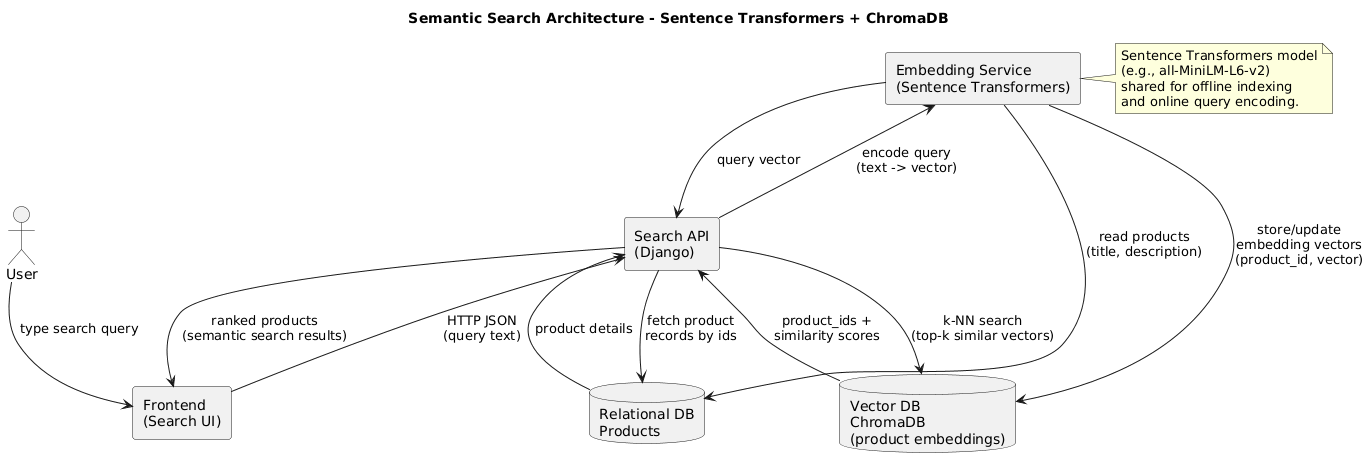
\includegraphics[width=0.9\textwidth]{Images/MyFigs/Semantic Search Architecture - Sentence Transformers + ChromaDB.png}
  \caption{Semantic search architecture using sentence transformers and ChromaDB for vector similarity retrieval.}
  \label{fig:semantic-search-architecture}
\end{figure}

\subsection{Recommendation Engine}
The recommendation engine is designed as a hybrid system combining content-based and simple collaborative signals.

\subsubsection*{Content-Based Recommendations}
Content-based recommendations rely on product similarity computed from text embeddings and structured attributes (e.g., category, brand). When a user views a product, the system retrieves:
\begin{itemize}
  \item products in the same or related categories;
  \item products with high cosine similarity in the embedding space;
  \item optionally, products matching known user preferences (e.g., price range).
\end{itemize}

\subsubsection*{Collaborative Filtering}
Collaborative filtering methods use historical interaction data (views, cart additions, purchases) to infer relationships between products and users. In \textit{ShopSense}, lightweight collaborative signals are used initially, such as:
\begin{itemize}
  \item ``users who viewed this also viewed'' based on co-viewing patterns;
  \item ``frequently bought together'' based on co-purchase counts when available.
\end{itemize}
These signals can be extended in future work with more advanced matrix factorization or neural models once sufficient data volume is available.

\subsubsection*{Hybrid Strategy}
The hybrid strategy combines content-based and collaborative scores to rank recommendations. A weighted linear combination is used in the initial implementation:

\begin{equation}
  \text{score}(p) = \alpha \cdot \text{sim}_{\text{content}}(p, p_{\text{ref}}) + (1 - \alpha) \cdot \text{score}_{\text{collab}}(p)
  \label{eq:hybrid-score}
\end{equation}

where:
\begin{description}
  \item[$p$] is the candidate product being evaluated for recommendation
  \item[$p_{\text{ref}}$] is the reference product (the product currently being viewed by the user)
  \item[$\text{sim}_{\text{content}}(p, p_{\text{ref}})$] is the cosine similarity between the embedding vectors of product $p$ and reference product $p_{\text{ref}}$, normalized to the range $[0,1]$
  \item[$\text{score}_{\text{collab}}(p)$] is the collaborative filtering score based on user interaction patterns (co-views, co-purchases), also normalized to $[0,1]$
  \item[$\alpha$] is a tunable weight parameter where $\alpha \in [0, 1]$. The default value is $\alpha = 0.7$, which emphasizes content-based similarity
\end{description}

\textbf{Adaptive Weighting Strategy:}
\begin{itemize}
  \item In cold-start scenarios (new products or insufficient collaborative data), the system sets $\alpha = 1.0$ to rely entirely on content-based similarity
  \item As interaction data accumulates over time, $\alpha$ can be reduced (e.g., to $0.6$ or $0.5$) to give more weight to behavioral signals
  \item This adaptive approach ensures sensible recommendations even with limited data while improving personalization as the system matures
\end{itemize}

Through this approach: 
\begin{itemize}
  \item sensible recommendations are provided even in cold-start scenarios (driven by content-based similarity);
  \item behavioral signals are gradually incorporated as data accumulates.
\end{itemize}

\section{Payment System Design}
Stripe, bKash, and a mock gateway are integrated by the payment subsystem to support the requirements identified in the problem statement. Secure handling of payment data and clear separation between order creation and payment confirmation are emphasized by the design.

\subsection{Stripe Integration Flow}
The Stripe payments were integrated for getting payment action done. The basic flow is illustrated in Figure~\ref{fig:stripe-flow}:
\begin{enumerate}[label=\roman*.]
  \item The customer selects card payment during checkout and submits the order details to the backend.
  \item The backend creates a payment intent or checkout session with Stripe, including amount, currency, and metadata (e.g., order ID).
  \item The frontend redirects the customer to Stripe’s secure payment page or uses Stripe’s client-side components to collect card details.
  \item Upon completion, Stripe sends a webhook to the backend indicating success or failure.
  \item The backend verifies the event, updates the order and payment status, and notifies the frontend.
\end{enumerate}

\begin{figure}[H]
  \centering
  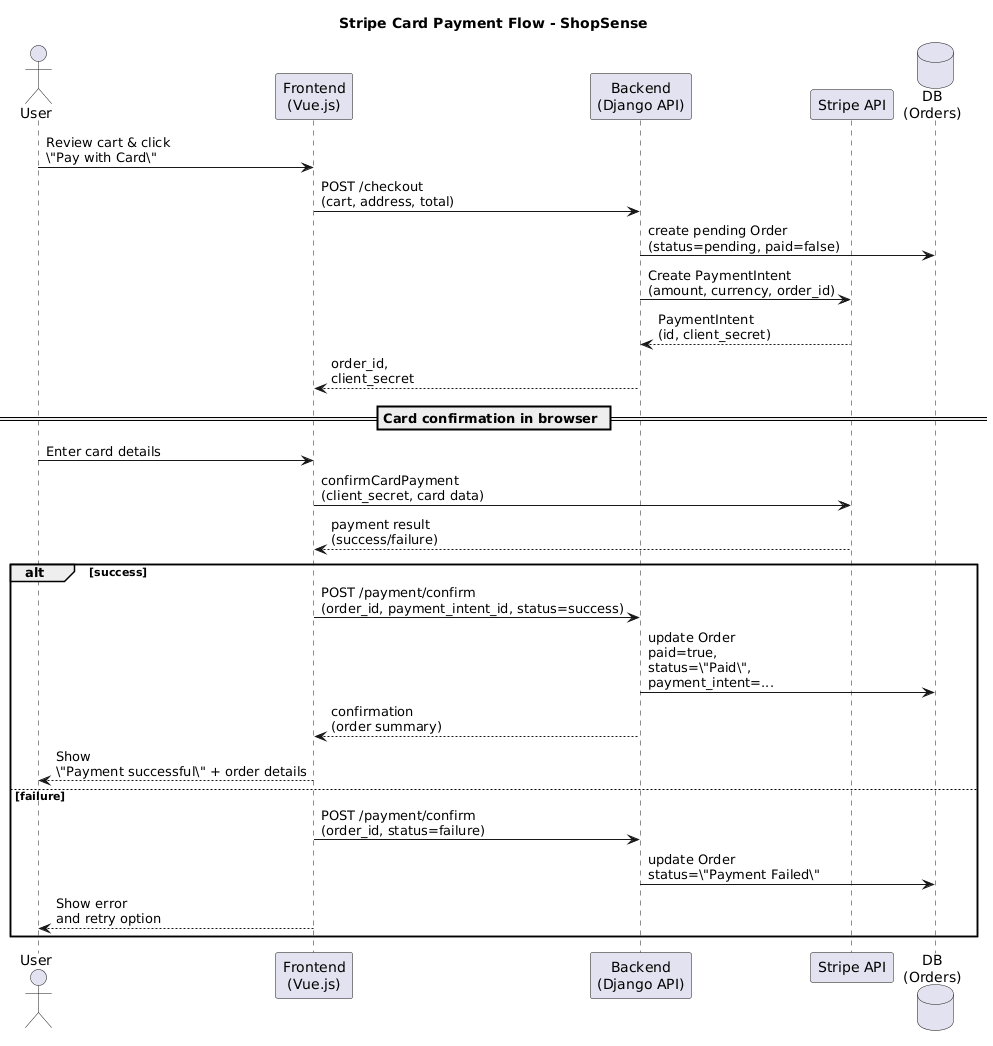
\includegraphics[width=0.9\textwidth]{Images/MyFigs/Stripe Card Payment Flow - ShopSense.png}
  \caption{Stripe payment integration flow for card payments in ShopSense.}
  \label{fig:stripe-flow}
\end{figure}

\subsection{bKash Integration Flow (Tokenized Checkout)}
The bKash integration follows the official tokenized checkout approach suitable for Bangladeshi merchants (Figure~\ref{fig:bkash-flow}):

\begin{enumerate}[label=\roman*.]
  \item The customer chooses bKash as the payment method and confirms the order on the checkout page.
  \item The backend authenticates with the bKash API to obtain an access token if one is not already available.
  \item The backend initiates a payment request with bKash, which returns a payment URL or token.
  \item The frontend redirects the customer to the bKash payment interface (web or app), where the customer authorizes the payment.
  \item bKash redirects back to the merchant callback URL or sends a notification with the payment result.
  \item The backend verifies the transaction status via the bKash API, updates the order and payment records, and informs the user.
\end{enumerate}

\begin{figure}[H]
  \centering
  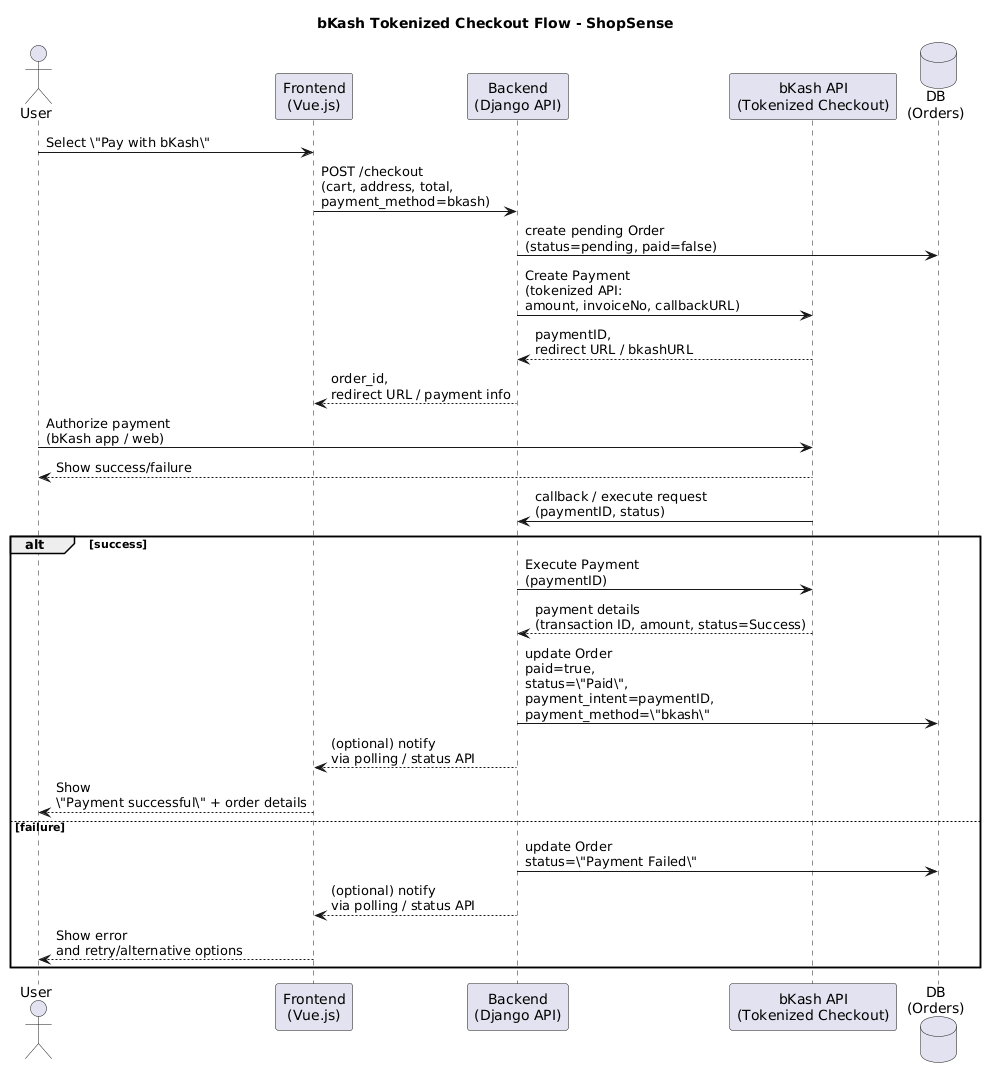
\includegraphics[width=0.9\textwidth]{Images/MyFigs/bKash Tokenized Checkout Flow - ShopSense.png}
  \caption{bKash checkout flow in ShopSense.}
  \label{fig:bkash-flow}
\end{figure}

\subsection{Mock Payment Gateway for Testing}
For testing purpose at the start I build a static gateway mimicking bKash sandbox to support development and demonstrations without relying on real payment providers. The mock gateway:
\begin{itemize}
  \item Provides some simple endpoints that mimicking the whole process for authorization, success, and failure situations;
  \item Instant approval or configurable delays/errors are allowed for testing.
  \item Structured responses similar to real gateways are returned so that the rest of the payment logic can be tested consistently.
\end{itemize}

Figure~\ref{fig:mock-payment-flow} provides an overview of the mock gateway flow.

\begin{figure}[H]
  \centering
  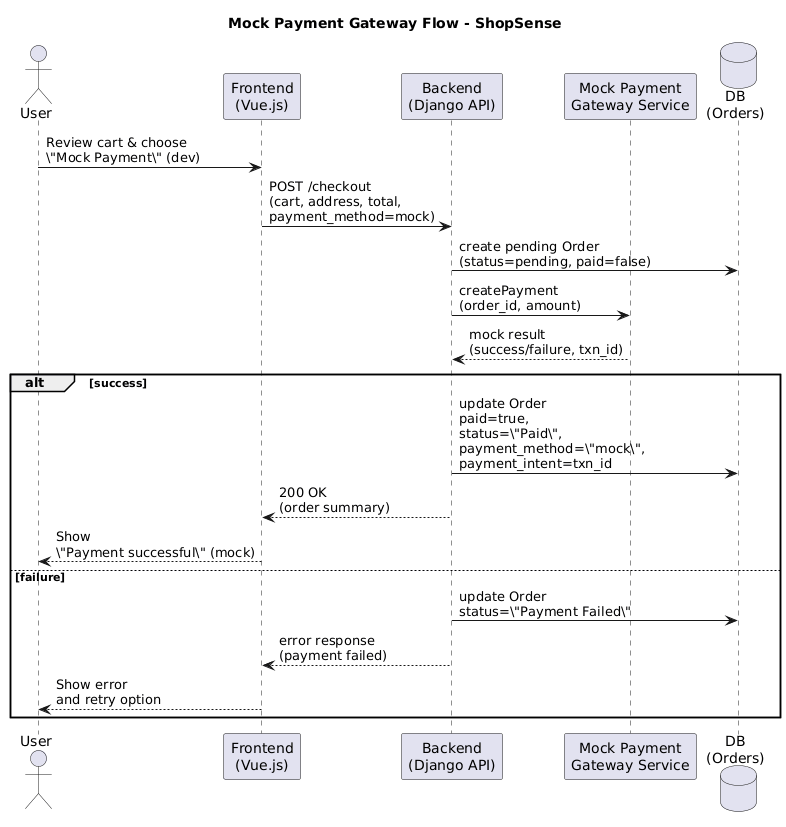
\includegraphics[width=0.9\textwidth]{Images/MyFigs/Mock Payment Gateway Flow - ShopSense.png}
  \caption{Mock payment gateway flow used for development and testing.}
  \label{fig:mock-payment-flow}
\end{figure}

\section{Security and Performance Considerations}
This section outlines how the system addresses security and performance concerns at a design level.

\subsection{Authentication, Authorization, CSRF}
\begin{itemize}
  \item \textbf{Authentication:} Django’s authentication framework is used to manage user logins, password hashing, and session management. For API calls, token-based or session-based authentication is used depending on the deployment configuration.
  \item \textbf{Authorization:} Access to administrative views and APIs is restricted by user roles and permissions. Regular users can only access their own profile and order data, while staff users can access management interfaces.
  \item \textbf{CSRF protection:} Django’s built-in CSRF middleware is enabled for state-changing operations. The Vue.js frontend includes CSRF tokens in relevant requests to prevent cross-site request forgery attacks.
  \item \textbf{Input validation and sanitization:} All external inputs (forms, API requests, webhook payloads) are validated on the server side. Where user-generated content is displayed, appropriate escaping and sanitization are applied.
\end{itemize}

\subsection{Static File Optimization, Caching, Database Tuning}
\begin{itemize}
  \item \textbf{Static file optimization:} Static assets (CSS, JavaScript, images) are collected via Django’s staticfiles framework and served through an optimized mechanism such as WhiteNoise or a CDN. Minification and bundling are applied on the frontend build pipeline to reduce payload size.
  \item \textbf{Caching:} Frequently accessed data (e.g., home page product lists, category menus) can be cached at the view or template level. API responses that do not change frequently may also be cached for short durations.
  \item \textbf{Database tuning:}We created appropriate indexes on the commonly queried fields things like product category, slug, and foreign keys. We also reviewed the query patterns to avoid any unnecessary joins or N+1 queries, especially when you're in the catalog and order-related views.
  \item \textbf{AI performance:} We optimized embedding generation and vector search by precomputing product embeddings and batching operations whenever possible. And in production deployments? And in production deployments, we can actually move those embedding and retrieval services to separate worker processes or servers.
\end{itemize}

So, ShopSense is ensured to remain secure, responsive, and maintainable by the combination of all the above measures. At the same time, advanced AI features and multi-payment integration are provided, making it perfect for those small to medium-scale deployments.


\section{Comparative Analysis with Existing Platforms}
Table~\ref{tab:platform-comparison} compares ShopSense with traditional e-commerce platforms and popular SaaS solutions, highlighting the unique value proposition and design choices of this work.

\begin{table}[H]
  \centering
  \caption{Comparison of ShopSense with existing e-commerce platforms.}
  \label{tab:platform-comparison}
  \small
  \begin{tabular}{|p{3.2cm}|p{3.2cm}|p{3.2cm}|p{3.2cm}|}
    \hline
    \textbf{Feature} & \textbf{Traditional BD Platforms} & \textbf{SaaS (Shopify)} & \textbf{ShopSense} \\
    \hline
    AI-Powered Semantic Search & Not available & Limited (via paid plugins) & Yes (built-in, ChromaDB + Sentence Transformers) \\
    \hline
    Recommendation Engine & Manual or none & Limited (basic tier) / Advanced (paid) & Yes (hybrid content + collaborative) \\
    \hline
    AI Chatbot (RAG-based) & External (Facebook Messenger, WhatsApp) & Third-party integrations only & Yes (integrated LangChain RAG) \\
    \hline
    Local Payment Integration (bKash) & Manual or semi-automated & Via third-party plugins & Native tokenized API integration \\
    \hline
    Card Payments (Stripe) & Rare or limited & Yes (standard) & Yes (full webhook support) \\
    \hline
    Cash on Delivery (COD) & Yes & Via apps & Yes (built-in) \\
    \hline
    Deployment Flexibility & Low (shared hosting) & None (SaaS only) & High (self-hosted, cloud-ready) \\
    \hline
    Customization & Limited by platform & Medium (theme + plugins) & High (full source code access) \\
    \hline
    Data Ownership & Full & Limited (vendor lock-in) & Full (self-hosted database) \\
    \hline
    Initial Setup Cost & Medium-High & Low (subscription starts \$29/mo) & Low (open-source, hosting cost only) \\
    \hline
    Scalability & Varies (often limited) & High (managed infrastructure) & Medium (configurable, horizontal scaling possible) \\
    \hline
    Analytics \& Reporting & Basic or none & Advanced (paid tiers) & Custom (extensible, raw data access) \\
    \hline
  \end{tabular}
\end{table}

\textbf{Key Observations:}
\begin{itemize}
  \item ShopSense addresses critical gaps in traditional Bangladeshi e-commerce platforms: intelligent product discovery, automated payment workflows, and conversational AI support
  \item Compared to SaaS solutions like Shopify, ShopSense offers greater control over data, lower long-term costs, and deeper customization capabilities suitable for SMEs with technical capacity
  \item The trade-off is that ShopSense requires self-hosting and maintenance, whereas SaaS platforms provide managed infrastructure
  \item For research and educational purposes, ShopSense demonstrates how open-source tools can achieve enterprise-grade features at a fraction of the cost
\end{itemize}

\section{Engineering Considerations}
This subsection discusses the engineering principles and design trade-offs that guided the development of ShopSense.

\subsection*{Scalability Considerations}
Several architectural decisions were made to support future scalability:

\begin{itemize}
  \item \textbf{Database indexing:} Indexes were created on frequently queried fields such as product \texttt{slug}, \texttt{category}, foreign keys (\texttt{product\_id}, \texttt{user\_id}), and \texttt{dateadded}. These indexes significantly reduce query latency for catalog browsing and order retrieval operations.
  
  \item \textbf{Caching strategy:} Django's caching framework is configured to support Redis or Memcached backends for:
  \begin{itemize}
    \item Session data (reducing database load)
    \item Frequently accessed views (e.g., homepage, category pages)
    \item API responses (e.g., cart count, product lists)
  \end{itemize}
  In the current prototype, file-based caching is used for simplicity, but production deployments can enable Redis with minimal configuration changes.
  
  \item \textbf{AI service separation:} Semantic search, recommendation computation, and chatbot inference are designed as loosely coupled modules. These can be deployed as:
  \begin{itemize}
    \item Separate Django management commands or Celery tasks for offline processing
    \item Independent microservices accessed via REST or gRPC APIs
    \item Containerized services orchestrated with Docker Compose or Kubernetes
  \end{itemize}
  
  \item \textbf{Horizontal scaling:} The Django backend is stateless (session data stored externally), allowing multiple application instances to be deployed behind a load balancer (e.g., Nginx, HAProxy, or cloud load balancers).
  
  \item \textbf{Static file delivery:} WhiteNoise serves static files efficiently in production. For high-traffic scenarios, static assets can be offloaded to a CDN (e.g., Cloudflare, AWS CloudFront).
\end{itemize}

\subsection*{Maintainability Considerations}
The codebase is structured to promote long-term maintainability:

\begin{itemize}
  \item \textbf{Modular app structure:} Django apps are organized by domain (store, cart, order, coupon, search, recommendations, chatbot, userprofile), promoting separation of concerns and making it easier to locate and modify functionality.
  
  \item \textbf{Configuration management:} Sensitive credentials and environment-specific settings are externalized using environment variables loaded via \texttt{python-dotenv}. This prevents hardcoding secrets and simplifies deployment across development, staging, and production environments.
  
  \item \textbf{Documentation:} Inline code comments, docstrings, and this thesis document provide comprehensive system documentation. API endpoints are self-documenting via Django REST Framework's browsable API interface.
  
  \item \textbf{Version control and CI/CD readiness:} The project is maintained in a Git repository with a clear branch strategy. The modular structure and automated tests (discussed in Chapter~4) facilitate continuous integration pipelines.
\end{itemize}

\subsection*{Extensibility Considerations}
The architecture is designed to accommodate future enhancements:

\begin{itemize}
  \item \textbf{RESTful API design:} Django REST Framework provides a stable, versioned API contract. Future clients (mobile apps, third-party integrations) can consume these APIs without requiring backend changes.
  
  \item \textbf{Payment gateway abstraction:} Payment methods are implemented with a common interface pattern. Adding new gateways (e.g., Nagad, Rocket) requires implementing the same interface without modifying existing checkout logic.
  
  \item \textbf{AI model swapping:} The chatbot supports configurable LLM backends (Ollama, OpenAI, mock) through environment variables and adapter classes. Similarly, embedding models can be swapped by changing the \texttt{SentenceTransformer} model name in configuration.
  
  \item \textbf{Plugin-ready architecture:} Future features such as product reviews, wishlists, or loyalty programs can be added as new Django apps without disrupting existing modules.
\end{itemize}

\subsection*{Technology Stack Justification}
The choice of technologies was driven by the following considerations:

\begin{itemize}
  \item \textbf{Django (Python):} Selected for rapid development, built-in ORM and admin interface, strong security features, and compatibility with Python's rich AI/ML ecosystem (PyTorch, Transformers, scikit-learn, LangChain).
  
  \item \textbf{Hybrid Vue.js frontend:} Embeds Vue~3 into Django templates rather than building a separate SPA. This approach:
  \begin{itemize}
    \item Eliminates the need for a complex frontend build pipeline
    \item Preserves server-side rendering benefits (SEO, faster initial page loads)
    \item Still provides modern reactive UI components (search bar, chatbot widget, cart badge)
  \end{itemize}
  
  \item \textbf{PostgreSQL:} Chosen for its reliability, ACID compliance, advanced indexing, JSON field support, and excellent Django integration. SQLite is used in development for simplicity.
  
  \item \textbf{ChromaDB:} A lightweight, embedded vector database suitable for prototype and small-to-medium scale deployments. For production scale, migration paths exist to Pinecone, Weaviate, or Qdrant.
  
  \item \textbf{Sentence Transformers:} Provides state-of-the-art sentence embeddings with reasonable computational requirements. Models like \texttt{all-MiniLM-L6-v2} balance accuracy and inference speed.
\end{itemize}

\subsection*{Design Trade-offs}
Several trade-offs were made during the design process:

\begin{itemize}
  \item \textbf{Hybrid frontend vs full SPA:} Sacrifices some client-side sophistication and component reusability for simpler deployment, better SEO, and lower infrastructure complexity. This is appropriate for small-to-medium merchants but may need revisiting for highly interactive or mobile-first applications.
  
  \item \textbf{Session-based cart:} Simpler to implement and suitable for the current scale, but does not support persistent carts across devices or long-term cart recovery. Migration to a database-backed cart model is straightforward if needed.
  
  \item \textbf{Lightweight AI models:} Prioritizes feasibility, response time, and resource efficiency over maximum accuracy. For example, \texttt{all-MiniLM-L6-v2} embeddings are sufficient for semantic search in a catalog of thousands of products, though larger models could improve performance with more computational resources.
  
  \item \textbf{Single-vendor design:} The current data model assumes a single merchant store. Supporting multi-vendor marketplaces would require significant extensions (vendor models, commission tracking, split payments) but the modular architecture provides a foundation for such growth.
  
  \item \textbf{Mock payment gateway:} Enables testing and demonstration without live credentials, but production deployments must replace mock flows with real gateway integrations and undergo security audits.
\end{itemize}

These engineering considerations demonstrate that ShopSense is not only functional but also architected with scalability, maintainability, and extensibility in mind, making it a solid foundation for real-world deployment and future research.

\section{Conclusion}
So, all the methodological approach and full system design of the \textit{ShopSense} webapp are discussed in this chapter. We actually developed the system step-by-step, using an iterative and Agile-inspired process, all based on clearly defined functional and non-functional requirements.\\
AI, front-end and backend design, overall architecture , user flow of the payment systems, and important security and performance issues? They are all discussed right here. And as for the next chapter? The process of implementing these designs and the technologies used to implement the platform are going to be detailed.

